%!TEX root = ../report.tex
\section{Hopf bifurcation}

Continuing on the upper branch of the pitchfork, we compute (at most) 6 of the eigenvalues closest to the origin after a few steps in $Re.$ After a while we find that a conjugate eigenpair crosses the imaginary axis, which indicates a Hopf bifurcation is nearby. The movement of the eigenvalues is visualized in Figure~...

\begin{figure}[h]
  \caption{A conjugate eigenpair crossing the imaginary axis.}
  \centerline{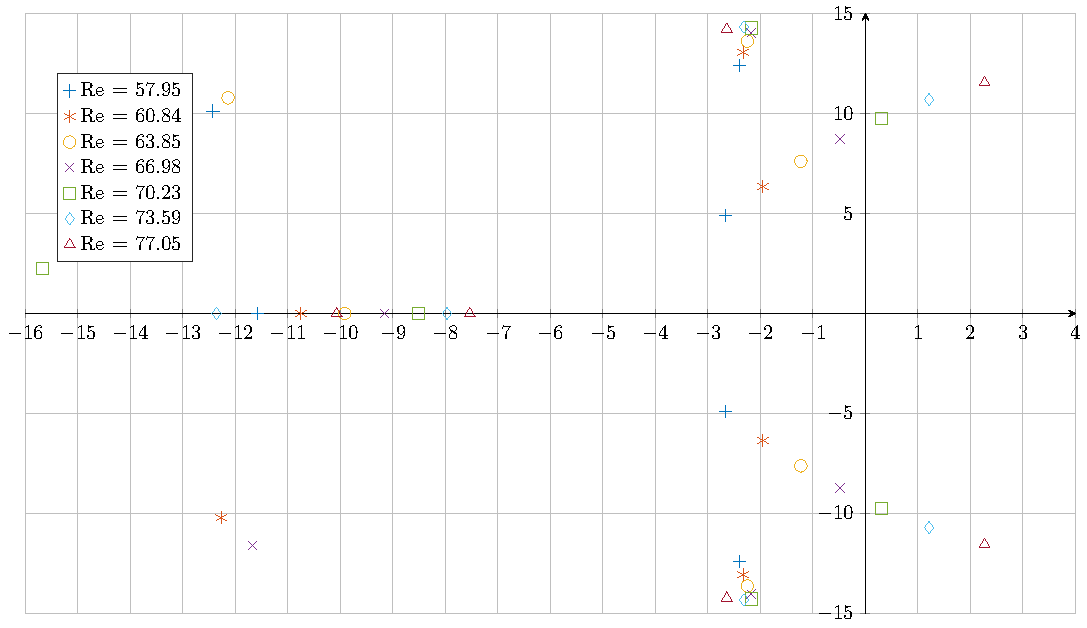
\includegraphics[width=\textwidth]{images/eigenwaarden_hopf.pdf}}
\end{figure}

Using the secant procedure to determine at which value of $Re$ the eigenpair is purely imaginary, we find that the Hopf bifurcation is located at $Re_H \approx 68.9781.$

